\chapter{Related Work}
\label{ch:state_of_the_art}
%
The ocean surface is an intricate phenomenon which owes its complexity
to its highly dynamic nature. Be it a quiet sea or an agitated one, small
turbulent waves or huge breaking ones, the underlying mechanisms are manifold
and act on a variety of scales. Oceanographic research defines the behaviour of
an ocean surface based on its location. Water areas far from the coast are
called~\emph{the deep ocean}, water areas close to shore are called
\emph{shallow water}. Deep ocean surfaces are governed by the interaction of
wind and gravity at the interface between air and water, whereas shallow water
surfaces are characterized by waves breaking near the shore.
%
\section{Simulation}
%
To date, computer graphics employs several ocean wave models which may be
separated roughly into three families: parametric description, spectral
description, computational fluid dynamics. The first describes the water surface
by means of parametric equations which have been derived based on real world
observations \citep{Gerstner:1809,Rankine:1863,Biesel:1952}.
The second family approximate the ocean surface using wave spectra which
simulate the sea as a random process based on the distribution of wave energy
in frequency space \citep{book:kinsman2002wind,article:PiersonMoskowitz1964,
article:Hasselman1973,article:Donelan1985,article:Elfouhaily1997}.
Third, computational fluid dynamics and more specifically the Navier-Stokes
equations are able to fully describe the dynamics of all kinds of fluid,
including the ocean.
%
\subsection{Parametric Models}
%
\begin{figure}
\centering
 \subtop
 {
  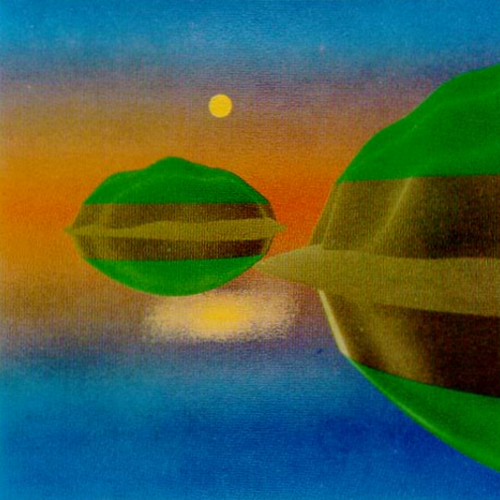
\includegraphics[scale=0.25]{figures/Vectorized_Procedural_Models_for_Natural_Terrain_-_Max_1981-006_1.png}
 }
 \hfill
 \subtop
 {
  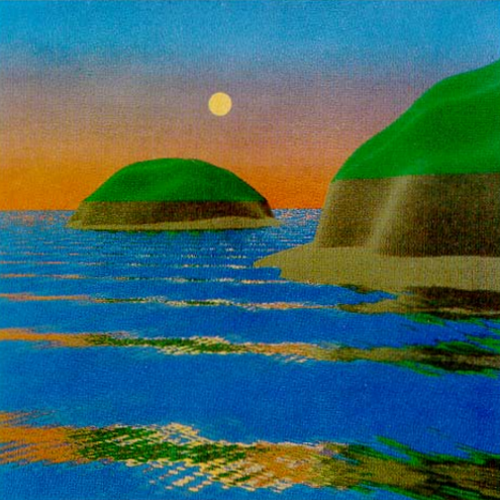
\includegraphics[scale=0.25]{figures/Vectorized_Procedural_Models_for_Natural_Terrain_-_Max_1981-007_1.png}
 }
 \hfill
 \subtop
 {
  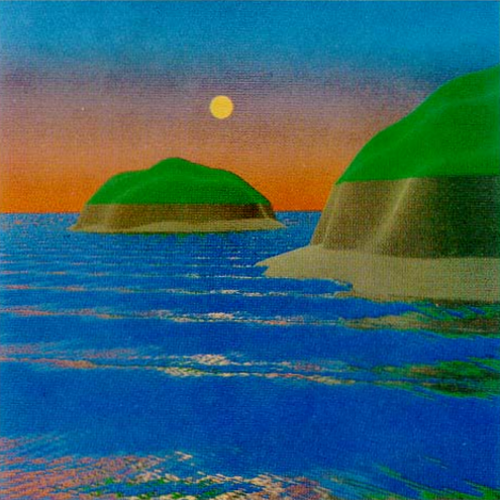
\includegraphics[scale=0.25]{figures/Vectorized_Procedural_Models_for_Natural_Terrain_-_Max_1981-006_2.png}
 }
 \hfill
 \subtop
 {
  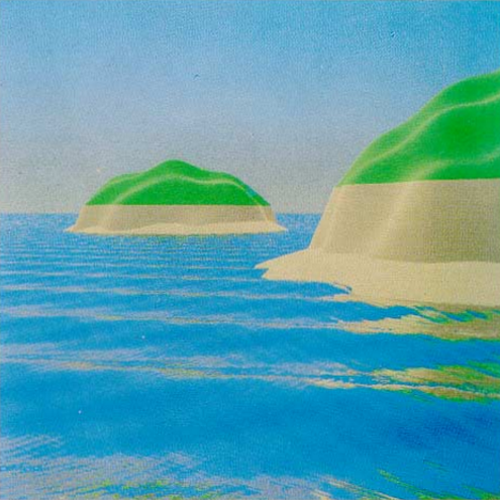
\includegraphics[scale=0.25]{figures/Vectorized_Procedural_Models_for_Natural_Terrain_-_Max_1981-007_2.png}
 }
\caption{Source:~\cite{Max:1981}}
\label{fig:max1981}
\end{figure}
%
The parametric models are generally bound to the spatial domain, where they
generate and animate the ocean surface by means of a sum of periodical functions
which evolve throughout time using a phase difference. One of the earliest works
in this realm of computer graphics has been done by~\citet{Max:1981}. The ocean
surface is represented as a height map, where for each point $(x,z)$ at time $t$
the height is computed as a sum of sinusoids:
\begin{equation}
h(x,z,t) = y + \sum_{i=1}^N A_i \cos (l_i x + m_i z - \omega_i t)
\end{equation}
where $y$ is the mean height of the free surface, $N$ is the number of waves,
$A_i$ is the amplitude of the $i$th wave, $\mvec{k}_i = (l_i, m_i)$ its wave
vector, and $\omega_i$ its angular frequency. The wave vector defines the
travelling direction of the wave, with the the positive X-axis pointing towards
the coastline, the Y-axis pointing in the opposite direction of earth's gravity,
and the Z-axis aligned with the coastline. For the sum of waves to achieve a
realistic shape, \citeauthor{Max:1981} applies linear wave theory.
The waves on the water surface are assumed to be dominated by gravity, the wave
amplitudes are assumed to be small in relation to the size of the water body,
and the water body is assumed to have infinite depth. According to linear
wave theory it follows that the wave vector $\mvec{k}$ and the angular frequency
$\omega$ are related by $\omega^2=kg$, where $k=\norm{\mvec{k}}$ and $g=9.81$
denotes earth's gravity. Results obtained by~\citeauthor{Max:1981} are shown in
Figure~\ref{fig:max1981}.
%
\begin{figure}
 \centering
 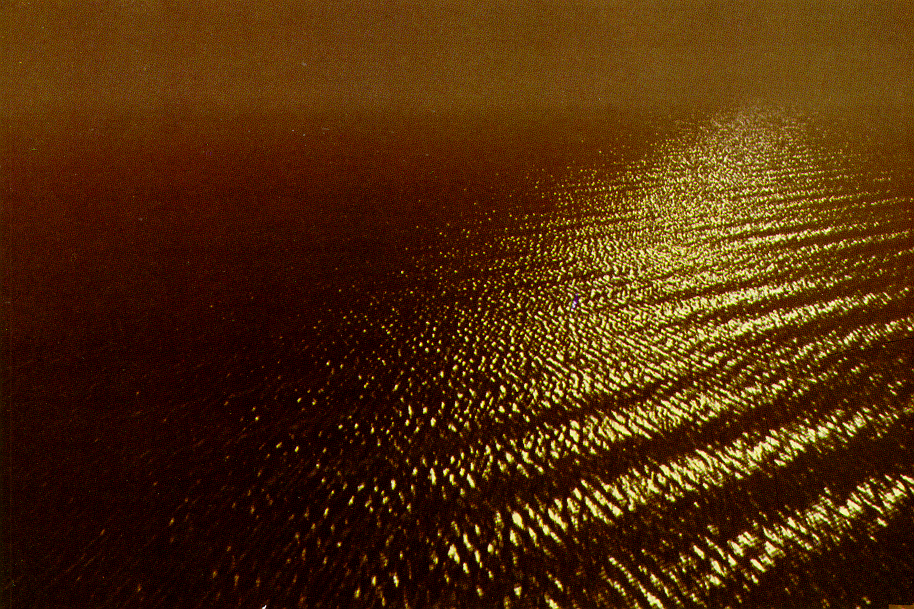
\includegraphics[scale=0.25]{figures/An_Image_Synthesizer_-_Perlin_1985-021.png}
 \caption{Perlin 1985}
\label{fig:perlin1985}
\end{figure}
%
Both,~\cite{Perlin:1985} and~\cite{Schachter:1980}
developed similar approaches, where instead of generating any actual geometry
they simply distorted the normal vectors of given surfaces using a variable
number of cycloids.

Spectral Models
Navier Stokes

Rendering

Particles
Reflection
Refraction
Foam, Sprays

Parametric\\
Perlin - An Image Synthesizer \cite{Perlin:1985}\\
Nelson Max - Vectorized Procedural Models for Natural Terrain: Waves and Islands in the Sunset \cite{Max:1981}\\
Peachey - Modeling Waves and Surf \cite{Peachey:1986}\\
Fournier - A simple model of ocean waves \cite{Fournier:1986}\\
Ts'o - Modeling and rendering waves: Wave-tracing using beta-splines and reflective and refractive texture mapping \cite{Ts'o:1987}\\Hinsinger - Interactive Animation of Ocean Waves \cite{Hinsinger:2002}\\

Spectral\\
Mastin - Fourier Synthesis of Ocean Scenes \cite{Mastin:1987}\\
Tessendorf - Simulating Ocean Water \cite{course:simulatingocean}\\
Premoze - Rendering Natural Waters \cite{Premoze:2000} \\

Hybrid\\
Thon - Ocean waves synthesis using a spectrum based turbulence function \cite{thon:2000}\\
Lee - Real-Time Simulation of Surface Gravity Ocean Waves Based on the TMA Spectrum\cite{lee:2007}\\



\begin{figure}
\centering
 \subtop
 {
  \includegraphics[scale=0.45]{figures/ocean300_5.jpg}
 }
 \hfill
 \subtop
 {
  \includegraphics[scale=0.45]{figures/ocean_storm300.jpg}
 }
\caption{The late afternoon sun illuminating the ocean surface. Source:~\cite{misc:noaa}}
\end{figure}



\begin{figure}
 \centering
 \subtop
 {
  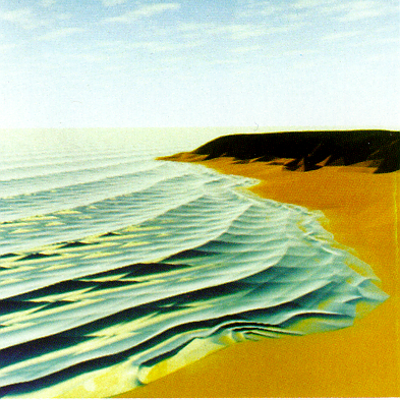
\includegraphics[scale=0.25]{figures/Modeling_Waves_and_Surf_-_Peachey_1986-009.png}
 }
 \hfill
 \subtop
 {
  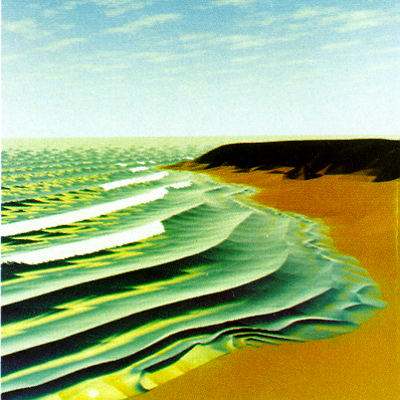
\includegraphics[scale=0.25]{figures/Modeling_Waves_and_Surf_-_Peachey_1986-010.png}
 }
 \hfill
 \subtop
 {
  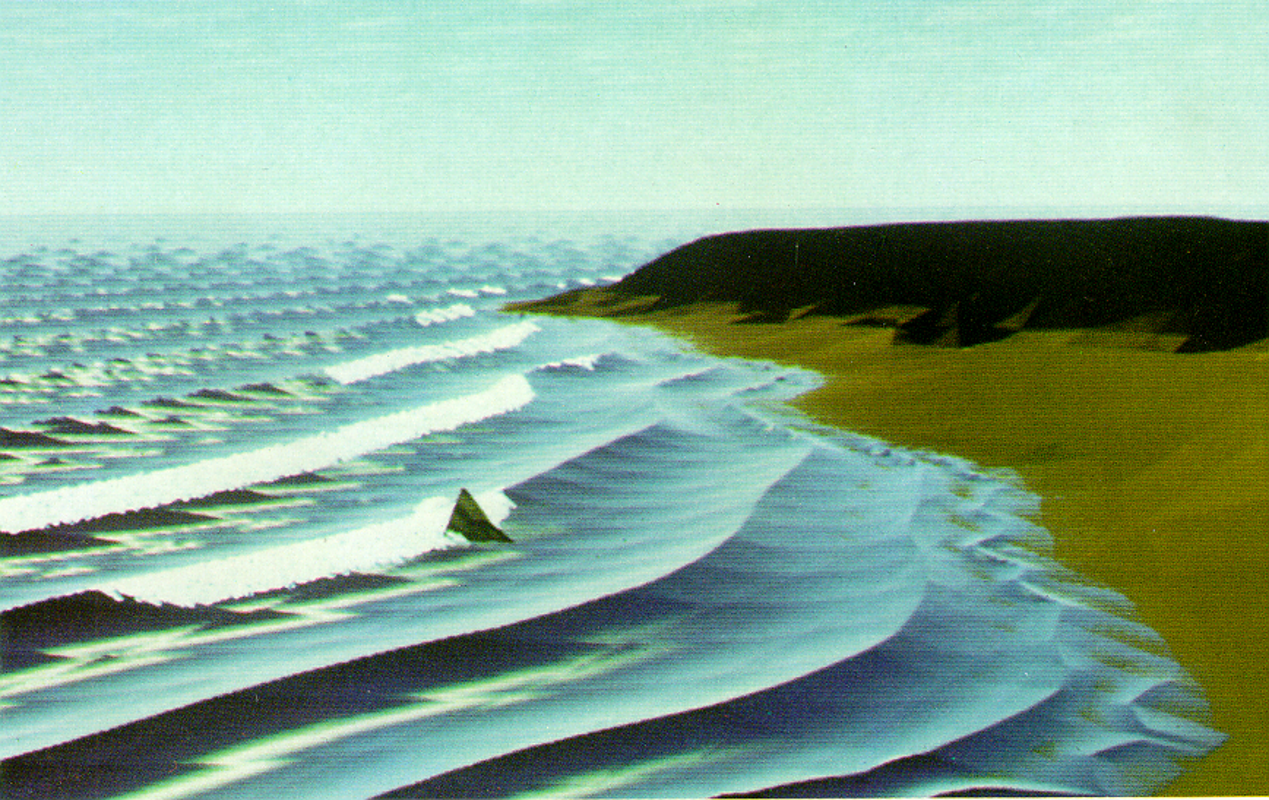
\includegraphics[scale=0.125]{figures/Modeling_Waves_and_Surf_-_Peachey_1986-012.png}
 }
 \caption{Peachey 1986}
\end{figure}

\begin{figure}
 \centering
 \subtop
 {
  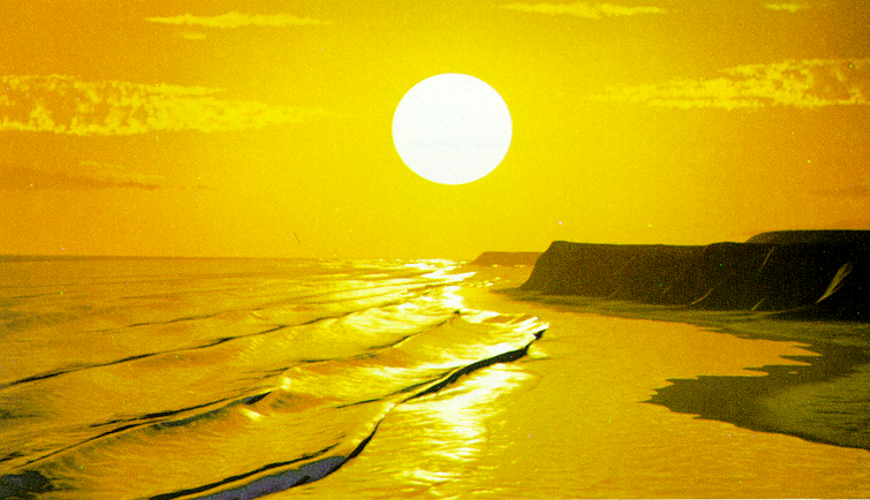
\includegraphics[scale=0.225]{figures/A_Simple_Model_of_Ocean_Waves_-_Fournier_1986-008.png}
 }
 \hfill
 \subtop
 {
  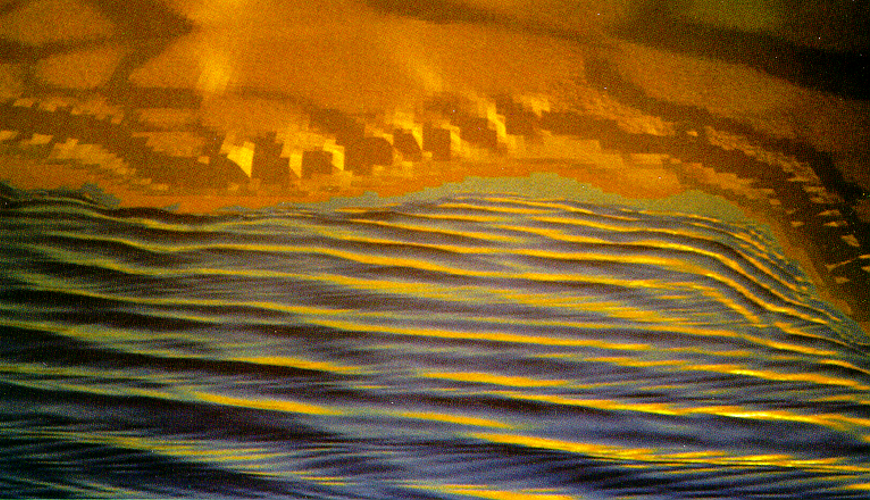
\includegraphics[scale=0.225]{figures/A_Simple_Model_of_Ocean_Waves_-_Fournier_1986-010.png}
 }
 \subtop
 {
  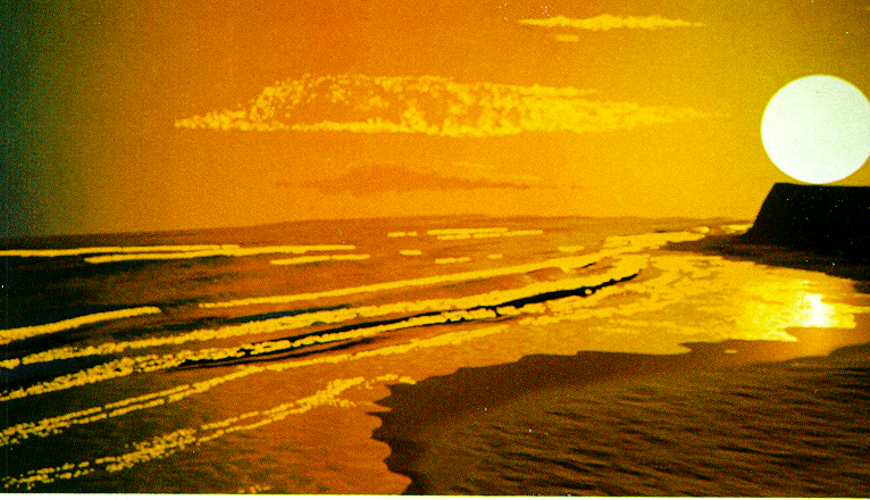
\includegraphics[scale=0.225]{figures/A_Simple_Model_of_Ocean_Waves_-_Fournier_1986-011.png}
 }
 \hfill
 \subtop
 {
  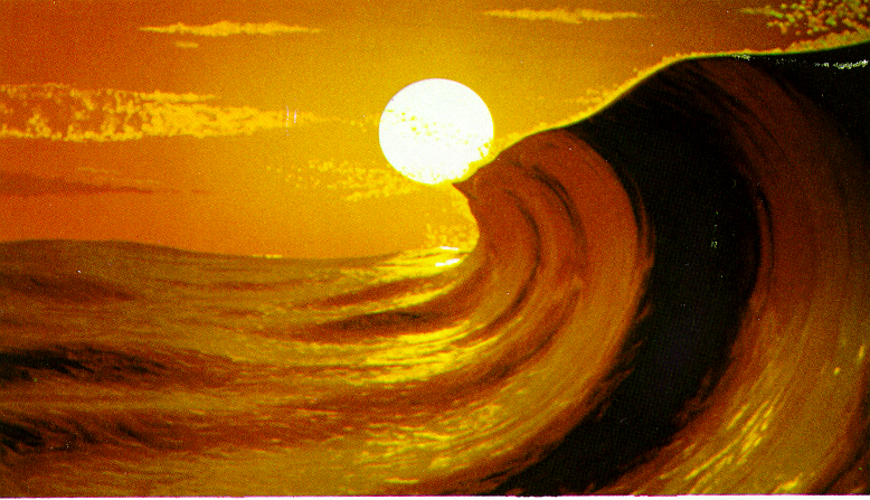
\includegraphics[scale=0.225]{figures/A_Simple_Model_of_Ocean_Waves_-_Fournier_1986-013.png}
	}
 \caption{Fournier 1986}
\end{figure}

\begin{figure}
 \centering
 \subtop
 {
  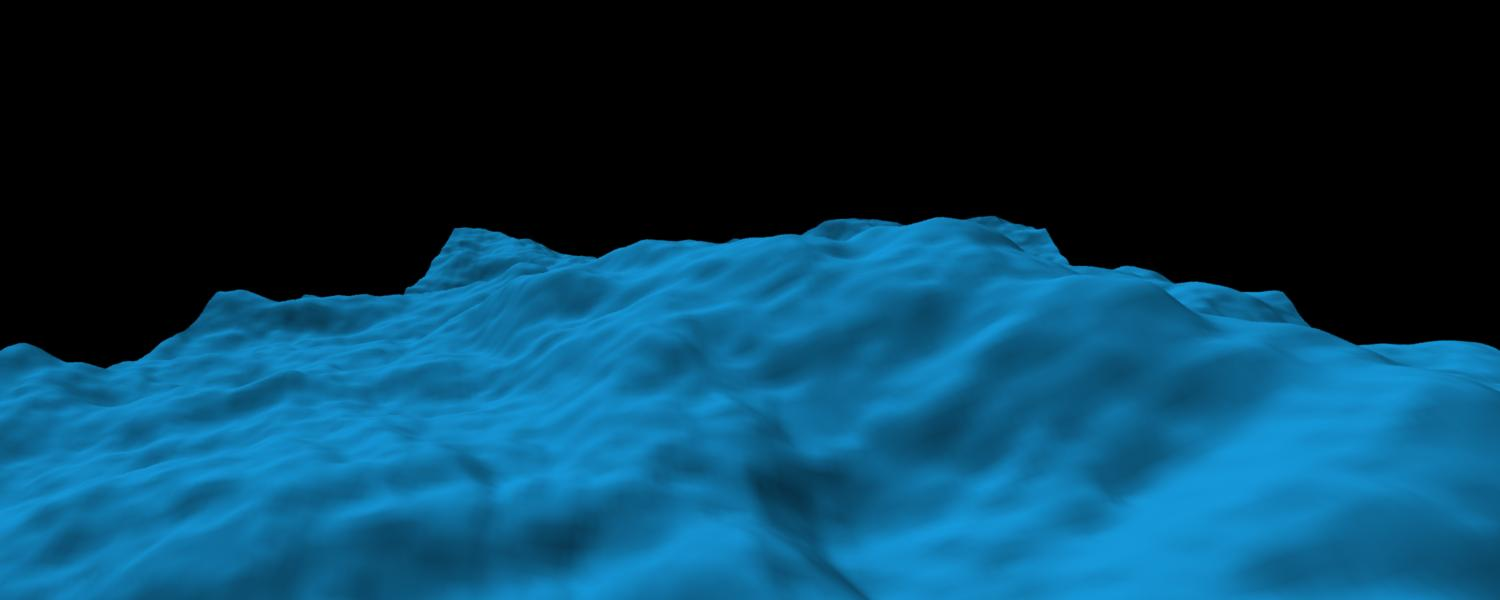
\includegraphics[scale=0.125]{figures/Simulating_Ocean_Water-012.png}
 }
 \subtop
 {
  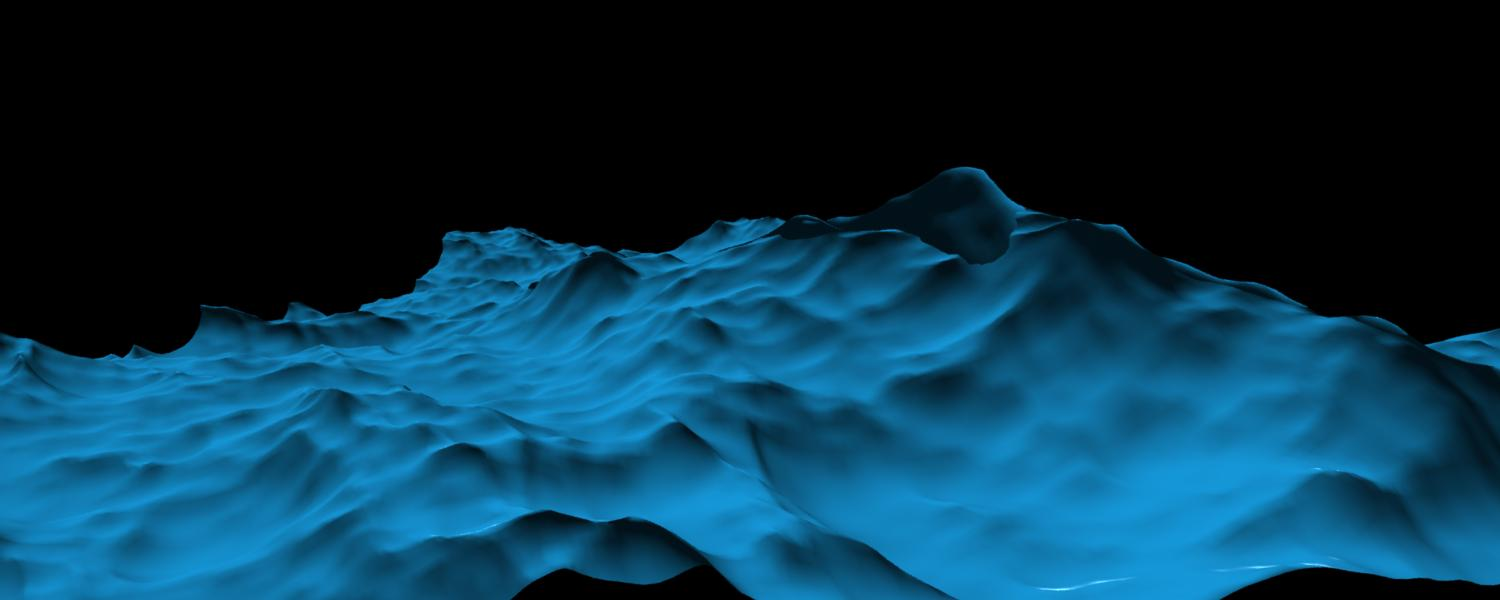
\includegraphics[scale=0.125]{figures/Simulating_Ocean_Water-013.png}
 }
 \caption{Tessendorf 1999}
\end{figure}

\begin{figure}
 \centering
 \subtop
 {
  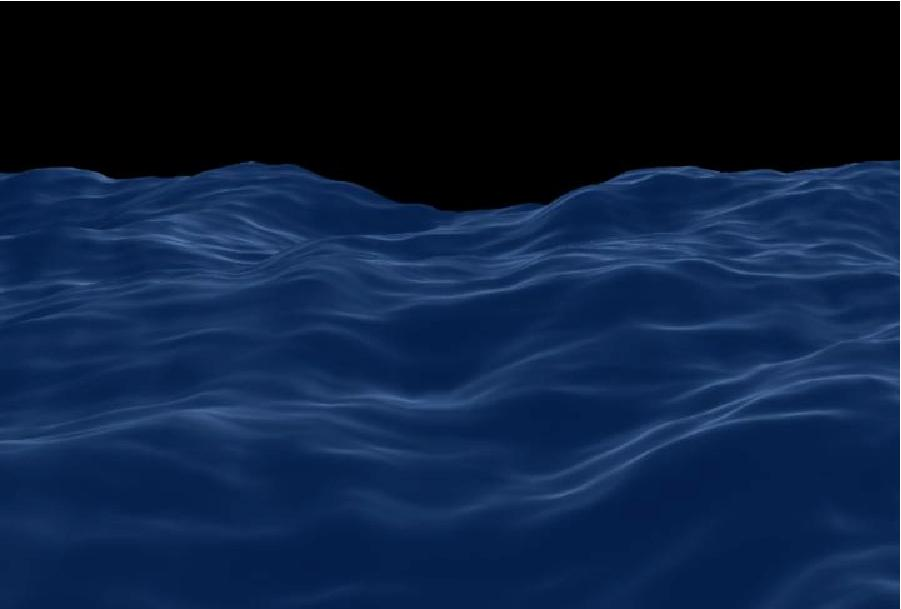
\includegraphics[scale=0.145]{figures/Simulating_Ocean_Water-008.png}
 }
 \hfill
 \subtop
 {
  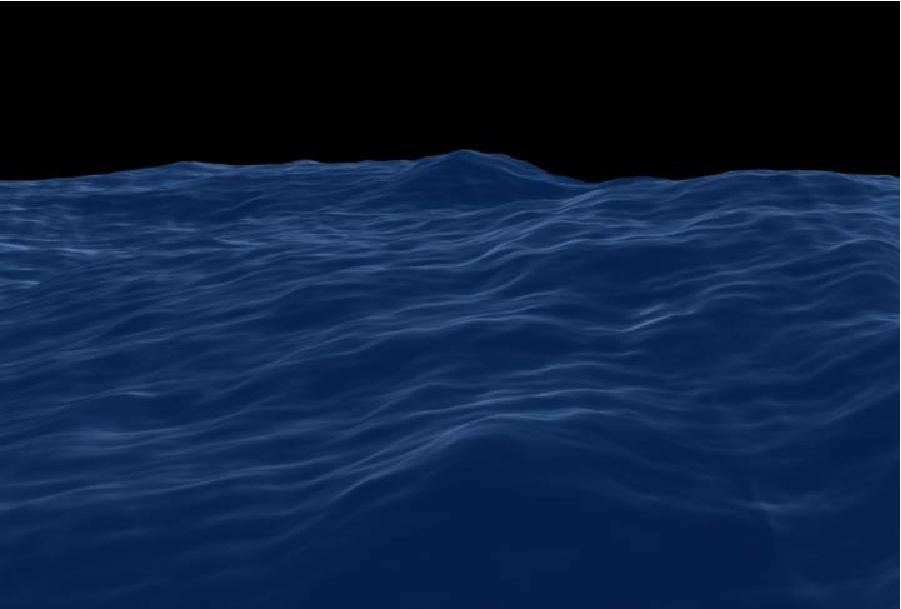
\includegraphics[scale=0.145]{figures/Simulating_Ocean_Water-009.png}
 }
 \hfill
 \subtop
 {
  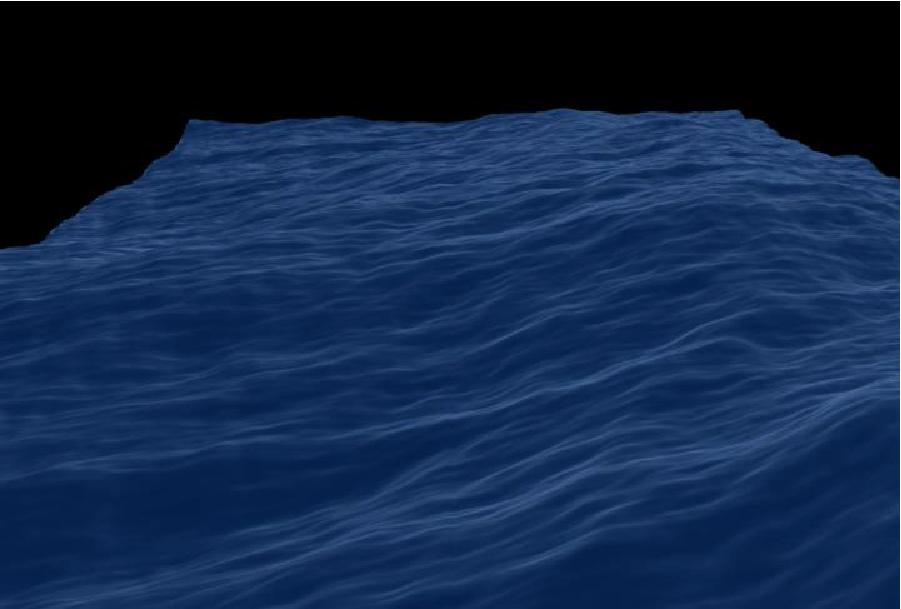
\includegraphics[scale=0.145]{figures/Simulating_Ocean_Water-010.png}
 }
 \caption{Tessendorf 1999}
\end{figure}